\documentclass{article}
\usepackage[utf8]{inputenc}
\usepackage{graphicx}
\usepackage{geometry}
\geometry{a4paper, total={16cm, 24cm}, top=2cm}
\usepackage{amsmath}
\usepackage{blindtext}
\graphicspath{ {img/} }
\usepackage{listings}
\usepackage{color}
\usepackage{hyperref}
\hypersetup{
    colorlinks=true,
    linkcolor=blue,
    filecolor=magenta,      
    urlcolor=cyan,
    }
\definecolor{dkgreen}{rgb}{0,0.6,0}
\definecolor{gray}{rgb}{0.5,0.5,0.5}
\definecolor{mauve}{rgb}{0.58,0,0.82}

\lstset{ frame=tb,
  language=C,
  aboveskip=3mm,
  belowskip=3mm,
  showstringspaces=false,
  columns=flexible,
  numbers=left,
  basicstyle={\small\ttfamily},
  numberstyle=\tiny\color{gray},
  keywordstyle=\color{blue},
  commentstyle=\color{dkgreen},
  stringstyle=\color{mauve},
  breaklines=true,
  breakatwhitespace=true,
  tabsize=3  
}


\title{Week 5 Programming Assignment}
\author{Steffen Petersen | au722120}
\date{October 3rd 2022}

\begin{document}
%\tableofcontents


\maketitle
\section{}
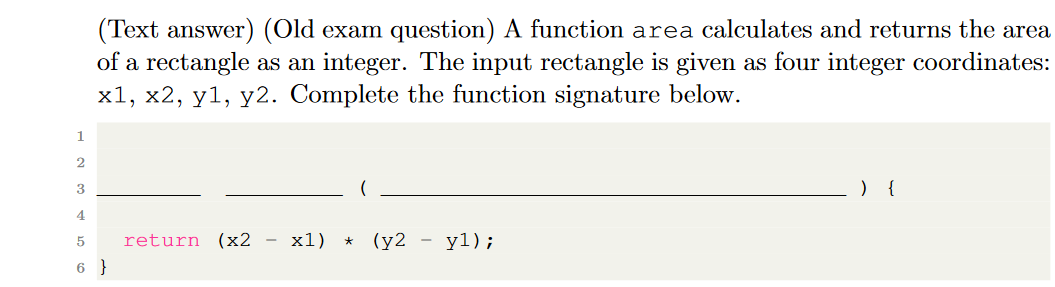
\includegraphics[width=\linewidth, keepaspectratio=true]{task1}
\vspace{2pt}\\
Bla


\section{}
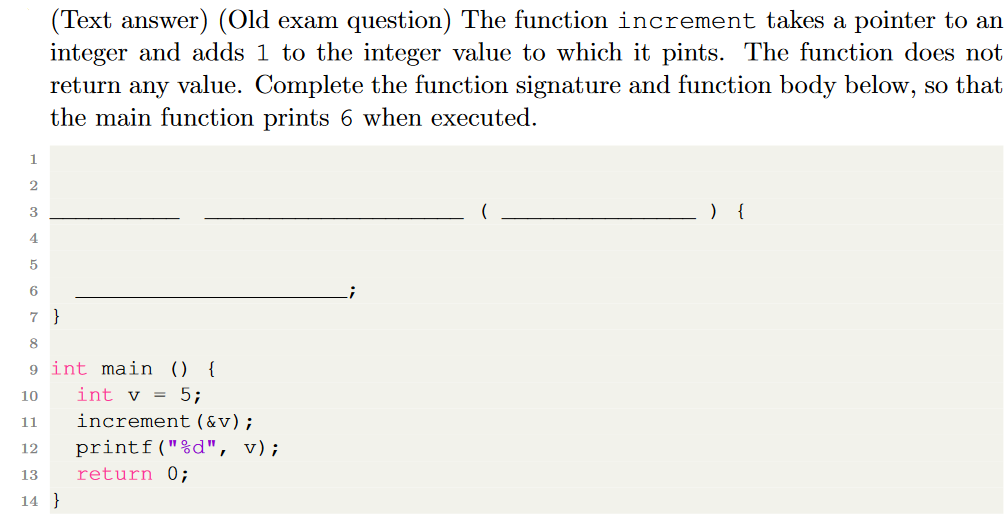
\includegraphics[width=\linewidth, keepaspectratio=true]{task2}
\vspace{2pt}\\




\section{}
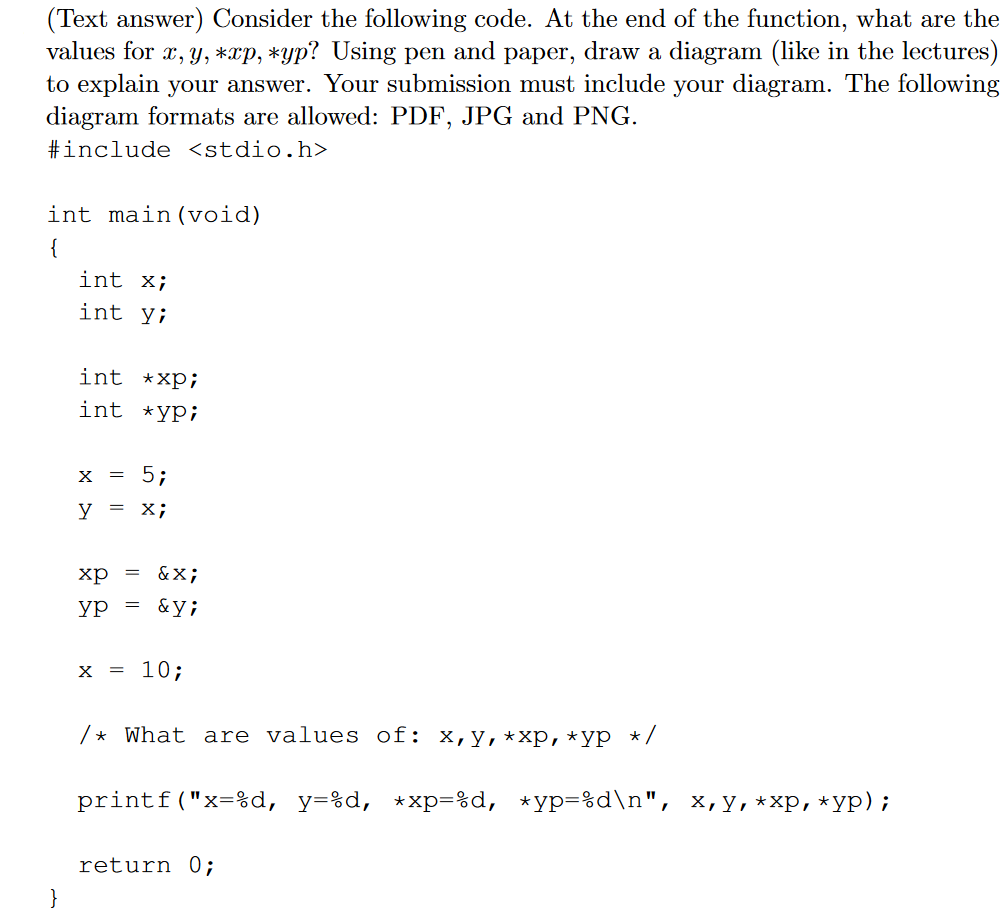
\includegraphics[width=\linewidth, keepaspectratio=true]{task3}
\vspace{2pt}\\

\section{}
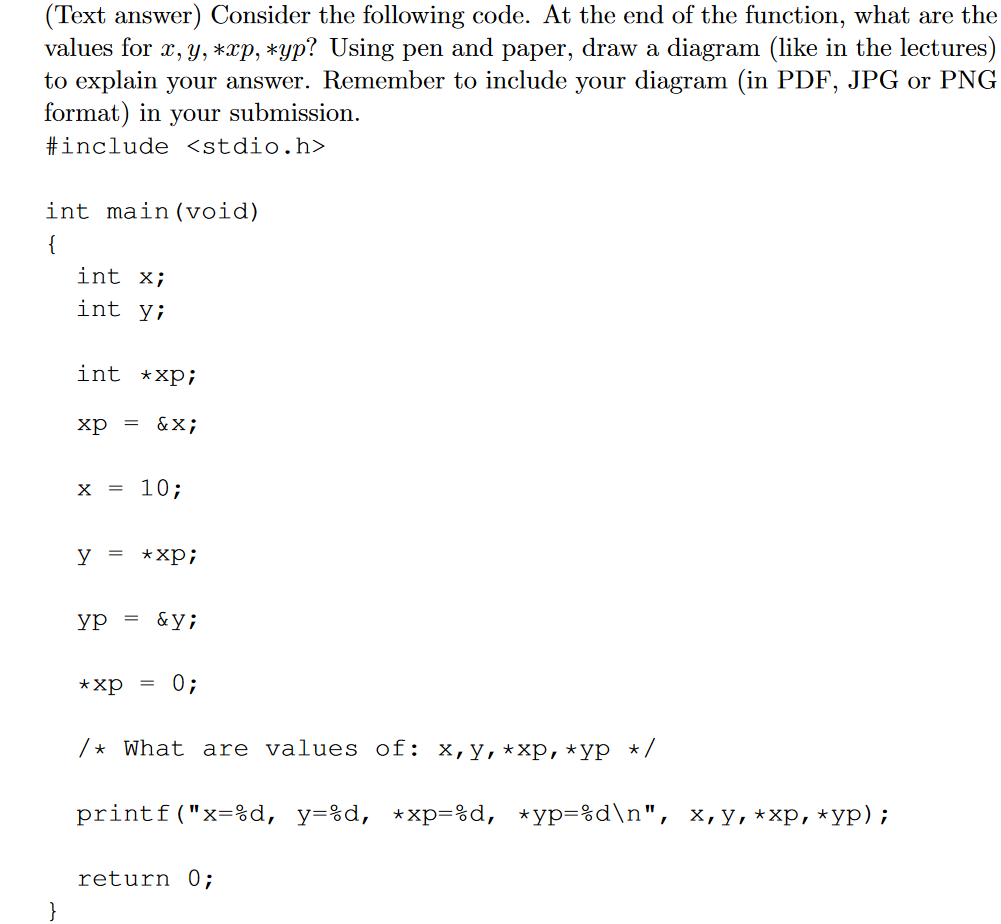
\includegraphics[width=\linewidth, keepaspectratio=true]{task4}
\vspace{2pt}\\


\section{}
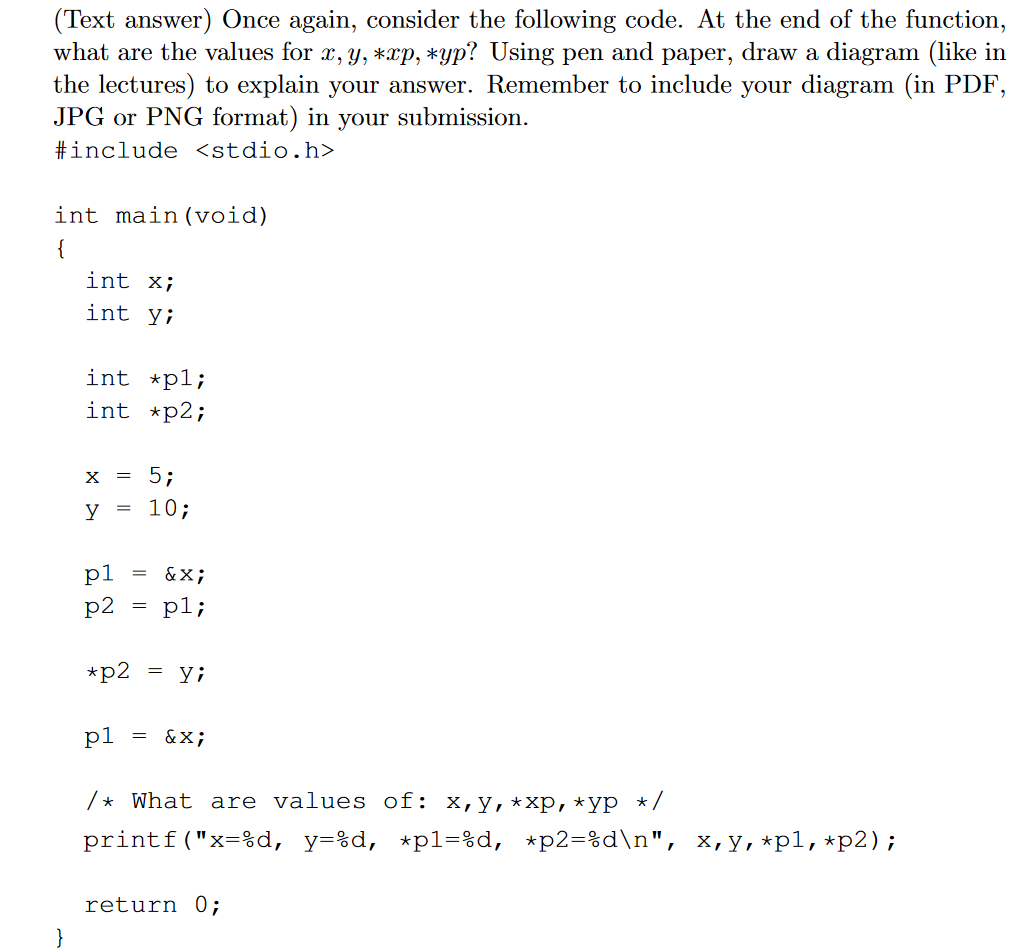
\includegraphics[width=\linewidth, keepaspectratio=true]{task5}
\vspace{2pt}\\
For this function I've used the return type double instead of void, as we would like to return the average value of the contents of the array, which double seems suitable for.\\
Below is my completed function, the same can be found in the task5.c file in the attached "Week 4 code.zip" folder, which includes a main function to test the average function.
\begin{lstlisting}
  double average(double list[], int n) // return type double to retain the best possible accuracy.
  {	
      double average; // Variable to store the ongoing sum and at last the average.
      for(int i = 0; i < n; i++){ 
          average += list[i];
      }
      average /= n; // Divide the sum of the whole array's values by its length, to get the average.
      return average;
  }
\end{lstlisting}


\section{}
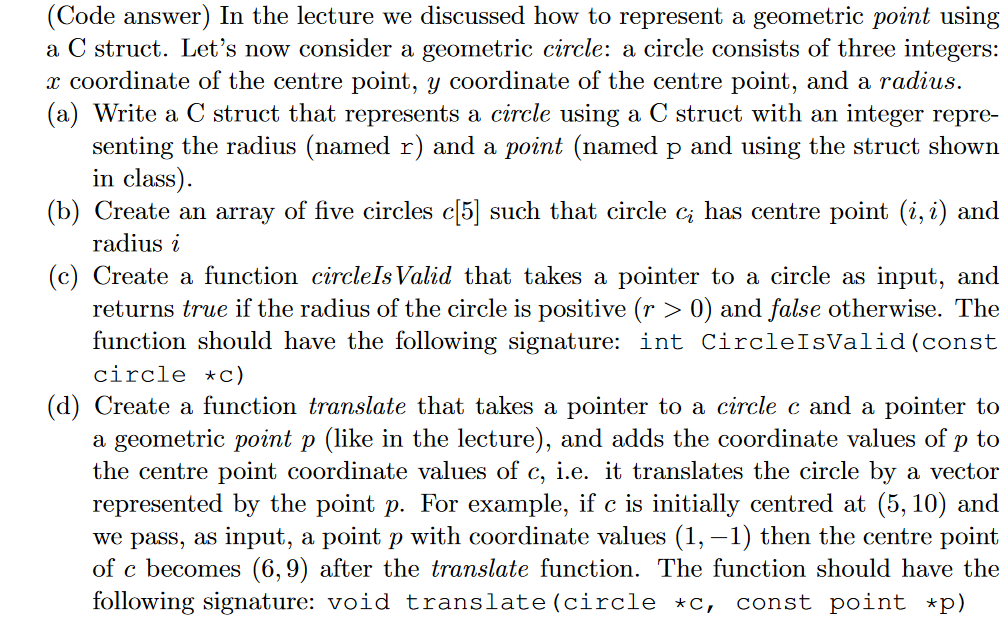
\includegraphics[width=\linewidth, keepaspectratio=true]{task6}
\vspace{2pt}\\



\section{}
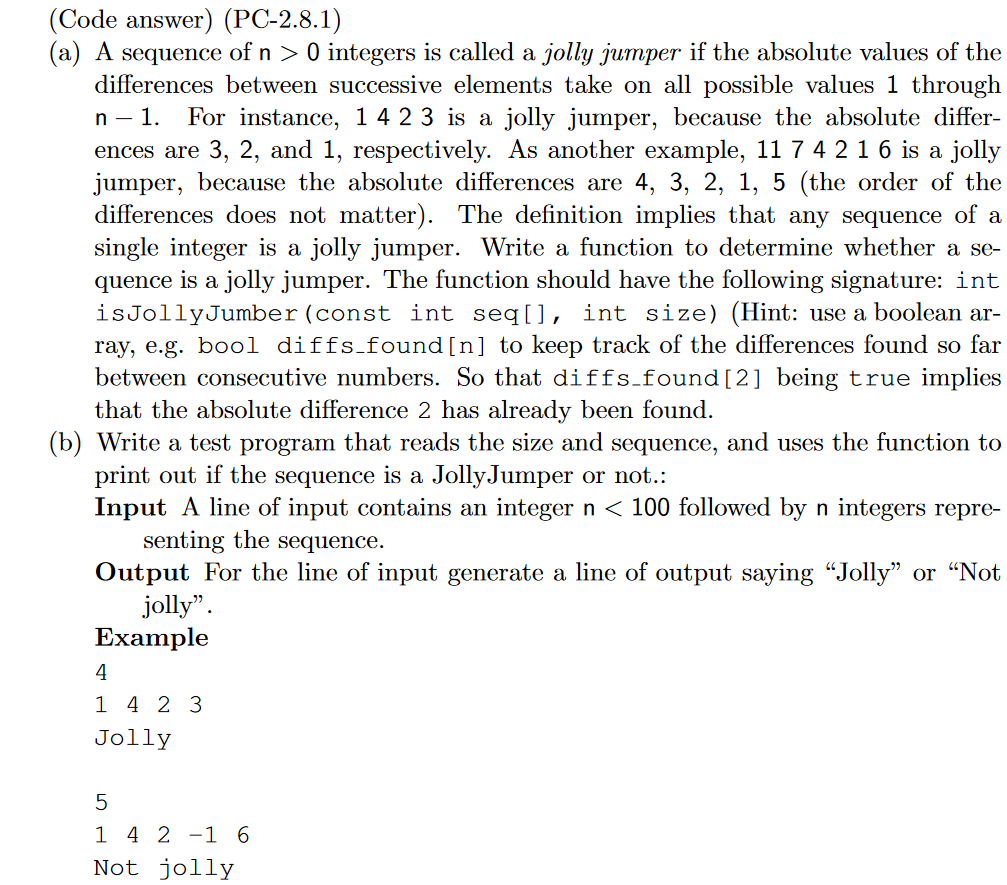
\includegraphics[width=\linewidth, keepaspectratio=true]{task7}
\vspace{2pt}\\


\end{document}